\documentclass{article}
\usepackage{tikz}
\usetikzlibrary{calc}
\begin{document}
\pagestyle{empty}
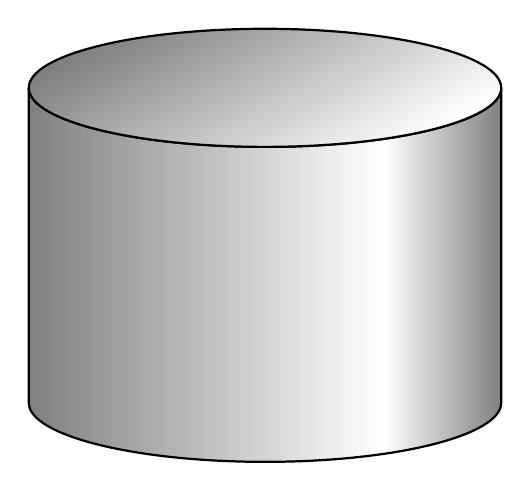
\begin{tikzpicture}    
   \coordinate (ll) at (-3,-2);
   \coordinate (lr) at (3,-2);
   \coordinate (ul) at (-3,2);
   \coordinate (ur) at (3,2);
   \shade [shading angle=90] (ll) arc (-180:-60:3cm and 0.75cm) -- +(0,4) arc (-60:-180:3cm and .75cm) -- cycle;
   \shade [shading angle=270] (lr) arc (0:-60:3cm and .75cm) -- +(0,4) arc (-60:0:3cm and .75cm) -- cycle;
   \draw [thick] (ll) arc (-180:0:3cm and 0.75cm) -- (ur) arc (0:-180:3cm and .75cm) -- cycle;
   \draw [thick, shade, shading angle=30] (ul) arc (-180:180:3cm and .75cm);

\end{tikzpicture}
\end{document} 
